%-----------------------------------
%
\chapter{Recipes}
%
%-----------------------------------

\AY{Different ways to put the above layers together/ordering them. Simulating RASPS and etc can go here?}


\section{Induction Heads}

\LS{Will write}

\section{Exchanging Heads for Layers}\label{sec:multihead}
We now show how one can exchange the computations performed by a transformer head with those of a transformer layer, assuming no layer normalization is performed.\AS{Check the layer norm thing}
This will allow us to focus on transformer constructions that only use heads, since those can be converted to layer-based ones.

Consider a transformer layer with $\nHead$ heads, where $\tfQ_h$, $\tfK_h$, and $\tfV_h$ are the query, key, and value transformations of the $h$\textsuperscript{th} head, respectively.
Intuitively, we will simply reuse the head's parameters as the parameters of the single head in a transformer block.
Since the head combining function $\headCombineFunc$ can look at the outputs of all the heads at once, we will also have to provide it with the outputs of all the heads at some point.
To enable this, we will make heavy use of the residual connections to accumulate the outputs of the layers that implement the individual heads.

Concretely, we define $\nHead$ transformer blocks with single heads---the head of $h$\textsuperscript{th} block will compute the transformation of the $h$\textsuperscript{th} head of the original block.
Supposing that each of the $\nHead$ heads computes $\hiddDim$-dimensional representations (with $\hiddDim'$-dimensional key and query vectors), we construct $\nHead$ layers working with $\left(\nHead + 1\right)\hiddDim$-dimensional representations.
The original input representations to the heads $\vx^{(0)}_1, \ldots, \vx^{(0)}_T \in \R^\hiddDim$ will be zero-padded to $\left(\nHead + 1\right)\hiddDim$ dimensions and each of the layers will then ``fill out'' one of the remaining $\nHead$ ``slots'' with the output of the corresponding head based on the input representations.
Schematically, denoting with $\mX^h$ the output of the $h$\textsuperscript{th} layer, one can think of the transformations performed by the $\nHead$ layers as follows:
\begin{subequations}
    \begin{align}
        \mX^0        & \colon \begin{pmatrix}
                                  \vx^{(0)}_1     & \vx^{(0)}_2     & \vx^{(0)}_3     & \cdots & \vx^{(0)}_{\tstep} & \cdots & \vx^{(0)}_T     \\
                                  \vzero_\hiddDim & \vzero_\hiddDim & \vzero_\hiddDim & \cdots & \vzero_\hiddDim    & \cdots & \vzero_\hiddDim \\
                                  \vzero_\hiddDim & \vzero_\hiddDim & \vzero_\hiddDim & \cdots & \vzero_\hiddDim    & \cdots & \vzero_\hiddDim \\
                                  \vdots          & \vdots          & \vdots          & \ddots & \vdots             & \ddots & \vdots          \\
                                  \vzero_\hiddDim & \vzero_\hiddDim & \vzero_\hiddDim & \cdots & \vzero_\hiddDim    & \cdots & \vzero_\hiddDim \\
                                  % 1               & 2               & 3               & \cdots & T               \\
                                  % 1               & 1               & 1               & \cdots & 1                     \\
                              \end{pmatrix}               \\
        \mX^1        & \colon \begin{pmatrix}
                                  \vx^{(0)}_1     & \vx^{(0)}_2     & \vx^{(0)}_3     & \cdots & \vx^{(0)}_{\tstep} & \cdots & \vx^{(0)}_T     \\
                                  \vx^{(1)}_1     & \vx^{(1)}_2     & \vx^{(1)}_3     & \cdots & \vx^{(1)}_{\tstep} & \cdots & \vx^{(1)}_T     \\
                                  \vzero_\hiddDim & \vzero_\hiddDim & \vzero_\hiddDim & \cdots & \vzero_\hiddDim    & \cdots & \vzero_\hiddDim \\
                                  \vdots          & \vdots          & \vdots          & \ddots & \vdots             & \ddots & \vdots          \\
                                  \vzero_\hiddDim & \vzero_\hiddDim & \vzero_\hiddDim & \cdots & \cdots             & \cdots & \vzero_\hiddDim \\
                                  % 1               & 2               & 3               & \cdots & T                     \\
                                  % 1               & 1               & 1               & \cdots & 1                           \\
                              \end{pmatrix}               \\
        \mX^2        & \colon \begin{pmatrix}
                                  \vx^{(0)}_1     & \vx^{(0)}_2     & \vx^{(0)}_3     & \cdots & \vx^{(0)}_{\tstep} & \cdots & \vx^{(0)}_T     \\
                                  \vx^{(1)}_1     & \vx^{(1)}_2     & \vx^{(1)}_3     & \cdots & \vx^{(1)}_{\tstep} & \cdots & \vx^{(1)}_T     \\
                                  \vx^{(2)}_1     & \vx^{(2)}_2     & \vx^{(2)}_3     & \cdots & \vx^{(2)}_{\tstep} & \cdots & \vx^{(2)}_T     \\
                                  \vdots          & \vdots          & \vdots          & \ddots & \vdots             & \ddots & \vdots          \\
                                  \vzero_\hiddDim & \vzero_\hiddDim & \vzero_\hiddDim & \cdots & \cdots             & \cdots & \vzero_\hiddDim \\
                                  % 1               & 2               & 3               & \cdots & T                     \\
                                  % 1               & 1               & 1               & \cdots & 1                           \\
                              \end{pmatrix}               \\
                     & \vdots   \nonumber                                                                                                                \\
        \mX^{\nHead} & \colon \begin{pmatrix}
                                  \vx^{(0)}_1      & \vx^{(0)}_2           & \vx^{(0)}_3      & \cdots & \vx^{(0)}_{\tstep}      & \cdots & \vx^{(0)}_T      \\
                                  \vx^{(1)}_1      & \vx^{(1)}_2           & \vx^{(1)}_3      & \cdots & \vx^{(1)}_{\tstep}      & \cdots & \vx^{(1)}_T      \\
                                  \vx^{(2)}_1      & \vx^{(2)}_2           & \vx^{(2)}_3      & \cdots & \vx^{(2)}_{\tstep}      & \cdots & \vx^{(2)}_T      \\
                                  \vdots           & \vdots                & \vdots           & \ddots & \vdots                  & \ddots & \vdots           \\
                                  \vx^{(\nHead)}_1 & \vx^{(\nHead)}_\nHead & \vx^{(\nHead)}_3 & \cdots & \vx^{(\nHead)}_{\tstep} & \cdots & \vx^{(\nHead)}_T \\
                              \end{pmatrix}
    \end{align}
\end{subequations}
Here, and $\vx^{(h)}_t$ is the output of the $h$\textsuperscript{th} head at position $t$.
To achieve this, we can the query, key, and value transformations of the $h$\textsuperscript{th} layer to be the same as the query, key, and value transformations of the $h$\textsuperscript{th} head of the original layer.
More concretely, let $\qproj_h \in \R^{\hiddDim' \times \hiddDim}, \kproj_h \in \R^{\hiddDim' \times \hiddDim}, \vproj_h \in \R^{\hiddDim \times \hiddDim}$ be the query, key, and value projection matrices of the $h$\textsuperscript{th} head of the original layer.\AS{handle the head MLPs}
Then, we define the query, key, and value projection matrices $\qproj_{L, h} \in \R^{\hiddDim' \times \left(\nHead + 1\right)\hiddDim}, \kproj_{L, h} \in \R^{\hiddDim' \times \left(\nHead + 1\right)\hiddDim}, \vproj_{L, h} \in \R^{\left(\nHead + 1\right)\hiddDim\times \left(\nHead + 1\right)\hiddDim}$ of the $h$\textsuperscript{th} layer as
\begin{subequations}
    \begin{align}
        \qproj_{L, h} = \begin{blockarray}{ccc}
                            \overbrace{\hspace{1.5cm}}^{\text{$\hiddDim$}} & \overbrace{\hspace{1.5cm}}^{\text{$\nHead \hiddDim$}} & \\
                            \begin{block}{(cc)c}
                \qproj_h & \mO_{\hiddDim' \times \nHead \hiddDim} & {\scriptstyle \hiddDim'} \\
            \end{block}
                        \end{blockarray} \\
        \kproj_{L, h} = \begin{blockarray}{ccc}
                            \overbrace{\hspace{1.5cm}}^{\text{$\hiddDim$}} & \overbrace{\hspace{1.5cm}}^{\text{$\nHead \hiddDim$}} & \\
                            \begin{block}{(cc)c}
                \kproj_h & \mO_{\hiddDim' \times \nHead \hiddDim} & {\scriptstyle \hiddDim'} \\
            \end{block}
                        \end{blockarray} \\
        \vproj_{L, h} = \begin{blockarray}{ccc}
                            \overbrace{\hspace{1.5cm}}^{\text{$\hiddDim$}} & \overbrace{\hspace{1.5cm}}^{\text{$\nHead \hiddDim$}} & \\
                            \begin{block}{(cc)c}
                \mO_{h \hiddDim \times \hiddDim} & \mO_{h \hiddDim \times \nHead \hiddDim} & {\scriptstyle h \hiddDim} \\
                \vproj_h & \mO_{\hiddDim \times \nHead \hiddDim} & {\scriptstyle \hiddDim} \\
                \mO_{\left(\nHead - h\right) \hiddDim \times \hiddDim} & \mO_{\left(\nHead - h\right) \hiddDim \times \nHead \hiddDim} & {\scriptstyle \left(\nHead - h\right) \hiddDim} \\
            \end{block}
                        \end{blockarray}.
    \end{align}
\end{subequations}
Each of the matrices $\qproj_{L, h}, \kproj_{L, h}, \vproj_{L, h}$ ``looks at'' the first $\hiddDim$ dimensions of the input representation to the layer (ones containing the original input representations to the heads).
This ensures that the $h$\textsuperscript{th} layer will compute the same transformation as the $h$\textsuperscript{th} head of the original layer and place it in the $h$\textsuperscript{th} ``slot'' of the output representation (which was previously zero-valued).
The MLPs can be set to implement the identity function.
Residual connections between the layers then ensure that the outputs of the heads are accumulated in the output of the layer.
At the end of the $\nHead$ layers, the $\nHead + 1$ ``slots'' thus contain the outputs of the $\nHead$ heads of the original layer and the input representations.
The MLP of the final layer can then combine these outputs to compute the final output of the layer by setting it to implement the head combining function $\headCombineFunc$.
This shows that the computations performed by transformer heads can be simulated by transformer layers, assuming no layer normalization is performed.

\section{\texorpdfstring{$n$}{n}-grams}

We now turn to the language modeling task (cf. \cref{sec:language-models}) and connect the transformer architecture to one of the simplest language model families: $n$-gram language models (\ngram{} LMs).
The next-symbol probabilities in \ngram{} LMs are computed under the \ngram{} assumption.
\begin{assumption}{\ngram{} Assumption}{ngram}
    The \defn{\ngram{} assumption} states that the conditional probability of the symbol $\sym_\tstep$ given $\strlt$ only depends on $n-1$ previous symbols $\str^{\tstep - 1}_{\tstep - n + 1} \defeq \sym_{\tstep-1},\ldots,\sym_{\tstep-n+1}$:\looseness=-1
    \begin{equation} \label{eq:n-gram-assumption}
        \plm\left(\sym_\tstep\mid \str_{<\tstep}\right) = \plm\left(\sym_\tstep \mid \str^{\tstep - 1}_{\tstep - n + 1}\right).
    \end{equation}
    \noindent We will refer to $\str^{\tstep - 1}_{\tstep - n + 1}$ as the \defn{history} of $\sym_\tstep$.
\end{assumption}

In the following, we describe how a transformer LM can simulate an \ngram LM in the sense of \cref{definition:lm-equivalence}.
We will need the following ingredients:
\begin{enumerate}[label=\textit{(\arabic*)}, topsep=5pt, itemsep=2pt,parsep=2pt]
    \item Hard attention (unique or averaging),
    \item No layer normalization,
    \item Unbounded positional encodings,
    \item Logarithmic precision,
    \item One-hot symbol encodings, and
    \item $n - 1$ heads.
\end{enumerate}


\begin{figure}
    \centering

    \begin{tikzpicture}[
        tape node/.style={draw=ETHBlue!80,minimum size=0.85cm,fill=ETHBlue!20},
        head node/.style={draw=ETHGreen!80,circle,minimum size=0.65cm,fill=ETHGreen!60,text=white},
        attn arrow/.style={-{Latex[length=2.25mm,width=1.5mm]},ETHGreen!100},
        comb arrow/.style={-{Latex[length=2.25mm,width=1.5mm]},ETHRed!70},
        comb node/.style={draw=ETHRed!80,circle,minimum size=0.75cm,fill=ETHRed!40},
        ]

        % Draw tape
        \foreach \i/\y in {0/$\sym_1$,1/$\sym_2$,2/$\cdots$,3/$\sym_{\tstep-4}$,4/$\sym_{\tstep-3}$,5/$\sym_{\tstep-2}$,6/$\sym_{\tstep-1}$,7/$\symt$,8/$\cdots$} {
                \ifnum \i=7
                    \node[tape node,fill=ETHBlue!40] (tape-\i) at (0.85*\i,0) {\footnotesize \y};
                \else
                    \ifnum \i>3
                        \ifnum \i<7
                            \node[tape node,fill=ETHBlue!25] (tape-\i) at (0.85*\i,0) {\footnotesize \y};
                        \fi
                    \else
                        \node[tape node,fill=ETHBlue!15] (tape-\i) at (0.85*\i,0) {\footnotesize \y};
                    \fi
                    \ifnum \i>7
                        \node[tape node,fill=ETHBlue!15] (tape-\i) at (0.85*\i,0) {\footnotesize \y};
                    \fi
                \fi
            }

        % Draw attention heads
        \node[head node] (head-1) at (2,1.7) {\scriptsize \texttt{Head 3}};
        \node[head node] (head-2) at (3.5,1.7) {\scriptsize \texttt{Head 2}};
        \node[head node] (head-3) at (5,1.7) {\scriptsize \texttt{Head 1}};

        % Draw arrows from heads to tape
        \draw[attn arrow, ETHGreen!20] (head-1) to[out=270,in=90] (tape-0.north);
        \draw[attn arrow, ETHGreen!20] (head-1) to[out=270,in=90] (tape-1.north);
        \draw[attn arrow, ETHGreen!20] (head-1) to[out=270,in=90] (tape-3.north);
        % \draw[attn arrow, ETHGreen!20] (head-1) to[out=270,in=90] (tape-4.north);
        \draw[attn arrow, ETHGreen!20] (head-1) to[out=270,in=90] (tape-5.north);
        \draw[attn arrow, ETHGreen!20] (head-2) to[out=270,in=90] (tape-0.north);
        \draw[attn arrow, ETHGreen!20] (head-2) to[out=270,in=90] (tape-1.north);
        \draw[attn arrow, ETHGreen!20] (head-2) to[out=270,in=90] (tape-3.north);
        \draw[attn arrow, ETHGreen!20] (head-2) to[out=270,in=90] (tape-4.north);
        % \draw[attn arrow, ETHGreen!20] (head-2) to[out=270,in=90] (tape-5.north);
        \draw[attn arrow, ETHGreen!20] (head-3) to[out=270,in=90] (tape-0.north);
        \draw[attn arrow, ETHGreen!20] (head-3) to[out=270,in=90] (tape-1.north);
        \draw[attn arrow, ETHGreen!20] (head-3) to[out=270,in=90] (tape-3.north);
        \draw[attn arrow, ETHGreen!20] (head-3) to[out=270,in=90] (tape-4.north);
        \draw[attn arrow, ETHGreen!20] (head-3) to[out=270,in=90] (tape-5.north);
        \draw[attn arrow] (head-1) to[out=270,in=90] (tape-4.north);
        \draw[attn arrow] (head-2) to[out=270,in=90] (tape-5.north);
        \draw[attn arrow] (head-3) to[out=270,in=90] (tape-6.north);

        % Draw combiner node
        \node[comb node] (combiner) at (4.5,3.4) {$\headCombineFunc$};

        % Draw arrows from tape to combiner
        \draw[comb arrow] (head-1.north) to[out=90,in=270] (combiner.south);
        \draw[comb arrow] (head-2.north) to[out=90,in=270] (combiner.south);
        \draw[comb arrow] (head-3.north) to[out=90,in=270] (combiner.south);

        \node[fill=none] (out) at (0.5,4.25) {$\plm\left(\symt\mid\strlt\right)$};

        % Draw an arrow from the combiner to the output
        % \draw[comb arrow] (combiner.north) -- ++(0,1.25) node[above] {};
        % \draw (combiner) edge[comb arrow, right] node{\footnotesize $\outMtx$} (out.south);
        \draw[comb arrow] (combiner.north) to[out=90,in=270] (out.south) ;
        % \node[fill=none] (out) at (3.45,3.7) {\footnotesize $\outMtx$};
        \node[fill=none] (out) at (3.2,4.5) {\footnotesize $\softmax\left(\outMtx \; \cdot\right)$};

    \end{tikzpicture}
    \caption{A transformer LM can simulate a $4$-gram LM using \textcolor{ETHGreen}{3 heads}. The stronger arrows from the heads to the symbols show where the heads focus their attention.}
    \label{fig:transformer-n-gram-label}
    \vspace{-10pt}
\end{figure}

The idea of the recipe is quite simple.
Given an $n$-gram LM $\plm$, we construct an equivalent transformer LM $\tfplm$ that looks back at the preceding $n - 1$ positions using the $n - 1$ heads, each of them uniquely attending to exactly one position.
The symbols attended to can be used to identify the full history, which can be used to access the conditional distribution over the next symbol.
This intuition is outlined in \cref{fig:transformer-n-gram-label}.\footnote{For simplicity, we disregard the role of residual connections in the following outline. Residual connections are, however, considered in the full proof later.}

To ease the exposition, we start with the final step of the construction: Assuming we have identified the appropriate history $\str^{\tstep - 1}_{\tstep - n + 1}$ after combining the head values using the head combining function $\headCombineFunc$, we show how $\tfplm$ can encode the conditional probability distribution $\plm\left(\sym_\tstep\mid\str_{\tstep- n + 1 : \tstep - 1}\right)$.
The intuition of this step is simple: Knowing what the individual $\plm\left(\sym_\tstep\mid\str^{\tstep - 1}_{\tstep - n + 1}\right)$ for $\sym_\tstep \in \eosalphabet$ are, we can simply put their logits into a vector and combine the constructed vectors for all possible histories into the output matrix $\outMtx$:\footnote{To be able to take the $\log$ of $0$ probabilities, we work over the set of \emph{extended} reals $\Rex = \R \cup \set{-\infty, \infty}$.}\textsuperscript{,}\footnote{Throughout the paper, we implicitly index the matrices directly with symbols and histories. We assume that the symbols and histories are ordered in some way and that the matrices are ordered accordingly.}
\begin{equation}
    \eOutMtx_{\sym, \str^{\tstep - 1}_{\tstep - n + 1}} \defeq \log{\plm\left(\sym_\tstep\mid\str^{\tstep - 1}_{\tstep - n + 1}\right)}
\end{equation}
In the following, we write $\tfenc\left(\strlt\right)$ as shorthand notation for $\tfenc\left(\strlt\right) \defeq \tfF\left(\vx_{\tstep - 1}^\nLayer\right)$ (i.e., the representation which is linearly transformed by $\outMtx$ to compute $\plm\left(\symt \mid \strlt\right)$ after normalization) where $\mX^\nLayer = \tf\left(\mX^0\right)\left(\strlt\right)$.
If we one-hot encode the identified history with $\tf$ as
\begin{equation}
    \tfenc\left(\strlt\right) \defeq \onehot{\str^{\tstep - 1}_{\tstep - n + 1}}
\end{equation}
we can then, using the formulation of the transformer LM from \cref{def:transformer-plnsm}, use the $\tfenc\left(\strlt\right)$ to look up the appropriate column in $\outMtx$ containing the logits of the conditional probabilities given the identified history for all possible $\sym_\tstep \in \eosalphabet$, i.e., $\left(\outMtx \ \tfenc\left(\strlt\right)\right)_\sym = \log\plm\left(\sym \mid\str^{\tstep - 1}_{\tstep - n + 1}\right)$.

We now consider the preceding step of the simulation: Identifying the history given that the $n - 1$ heads identified the symbols $\sym_1, \ldots, \sym_{n - 1}$ in the positions they attended to.
If we concatenate the values of the $n - 1$ heads into a vector $\vv$, this vector of size $\left(n - 1\right)|\eosalphabet|$ will contain the \defn{multi-hot} representation of the history of interest:
\begin{equation}
    \vv = \begin{pmatrix}
        \onehot{\sym_1} \\
        \vdots          \\
        \onehot{\sym_{n - 1}}
    \end{pmatrix}
\end{equation}
and $\vv_{i |\eosalphabet| + j} = 1$ if and only if $r\left(\sym_i\right) = j$ for a bijection $r\colon \eosalphabet \to \NTo{|\eosalphabet|}$ that determines the indices of the one-hot representations of the symbols.
We would then like to transform this vector into a vector $\vu \in \R^{|\alphabet|^{n - 1}}$ such that
\begin{equation}
    \evu_{i} = 1 \iff i = r'\left(\sym_1, \ldots, \sym_{n - 1}\right)
\end{equation}
for a bijection $r'\colon \underbrace{\eosalphabet \times \cdots \times \eosalphabet}_{n - 1\text{ times}} \to \NTo{|\eosalphabet|^{n - 1}}$.
This can be equivalently written as
\begin{equation}
    \evu_{i} = 1 \iff \evv_{j |\eosalphabet| + r\left(\sym_j\right)} = 1 \text{ for all } j = 1, \ldots, n - 1
\end{equation}
where $i = r'\left(\sym_1, \ldots, \sym_{n - 1}\right)$.
This is an instance of performing the logical \texttt{AND} operation, which can be implemented by an MLP as described in \cref{sec:ffnn_boolean}.
This MLP will form the transformation $\headCombineFunc$ combining the information obtained from all the heads of the transformer.

This brings us to the final part of the proof: Identifying the symbols at the previous $n - 1$ positions by the $n - 1$ transformer heads.
To show how this can be done, let us consider the parameters we can still set to define a transformer:
\begin{itemize}
    \item The static symbol representations $\statRep$ and the positional encodings $\posEnc$.
          For static representations, we use simple one-hot encodings $\onehot{\sym}$: $\statRepFun{\sym} \defeq \onehot{\sym}$.
          For positional encodings, we use the following function:
          \begin{equation}
              \posEncFun{\tstep} = \begin{pmatrix}
                  \tstep - h \\
                  1
              \end{pmatrix} \in \R^{2}
          \end{equation}
          We concatenate $\statRep$ and $\posEnc$ to obtain the symbol representations $\posStatRepFun{\sym_\tstep, \tstep} \in \R^{\nsymbols + 2}$.
    \item The attention scoring function $\tfScore$.
          We will use the a slightly modified version of the standard dot-product scoring function:
          \begin{equation} \label{eq:transformer-ngram-function}
              \tfScore\left(\vq, \vk\right) \defeq -\abs{\innerProd{\vq}{\vk}}.
          \end{equation}
          $\tfScore$ will, together with the positional encodings, allow us to easily single out the relevant positions in the string.
    \item The parameters of each of the attention heads, that is, the transformations $\tfQ$, $\tfK$, and $\tfV$.
          Each of those will take the form of a linear transformation of the static representations.
          We describe them in more detail below.
\end{itemize}
The parameters of all the heads will be identical, with the only difference being a single parameter that depends on the ``index'' of the head, $h \in \NTo{\nHead}$.
We describe the individual transformations $\tfQ_h$, $\tfK_h$, $\tfV_h$, and $\tfO_h$ of the head $h$.
At any time step $\tstep$ (i.e., when computing the conditional distribution $\plm\left(\sym_\tstep \mid \strlt\right)$), the head $h$ will attend to the symbol at position $\tstep - h$, $\sym_{\tstep - h}$.
In \cref{fig:transformer-n-gram-label}, for example, \texttt{Head $3$} attends to the position $\tstep - 3$, which is denoted by the stronger arrow to that position.
We want it to put all its attention to this position: Given the query $\vq_{\tstep - 1}$, we want the attention function in \cref{eq:transformer-ngram-function} to be uniquely maximized by the key of the symbol at position $\tstep - h$.
Notice that, therefore, the key does not have to depend on the identity of the symbol at position $\tstep - h$---only the positional information matters.
We consider the following query and key transformations for head $h$:
\begin{align}
    \tfQ_h\colon & \begin{pmatrix}
                       \onehot{\symt} \\
                       \tstep - h     \\
                       1
                   \end{pmatrix} \mapsto \begin{pmatrix}
                                             \tstep - h \\
                                             -1
                                         \end{pmatrix} \\
    \tfK_h\colon & \begin{pmatrix}
                       \onehot{\symt} \\
                       \tstep - h     \\
                       1
                   \end{pmatrix} \mapsto \begin{pmatrix}
                                             1 \\
                                             \tstep
                                         \end{pmatrix}.
\end{align}
Both are clearly linear.
Intuitively, both transformations keep only the positional information.
The query transformation ``injects'' the knowledge of which position should maximize the attention score, while the key transformation simply ``exposes'' the positional information about the symbol.
The constants $1$ and $-1$ and the index of the position ensure that the inner product simply computes the difference between the position of the symbol and the position of interest:
\begin{equation} \label{eq:hard-attention-scores}
    \tfScore\left(\vq_\tstep, \vk_j\right) = \innerProd{\begin{pmatrix}
            \tstep - h \\
            -1
        \end{pmatrix}}{\begin{pmatrix}
            1 \\
            j
        \end{pmatrix}} = -\abs{j - \tstep + h},
\end{equation}
which is maximized by $j = \tstep - h$.

This leaves us with the question of how to use the position of the symbol of interest ($\tstep - h$) to extract the one-hot encoding of the symbol at that position.
Due to the information contained in the symbol representations $\posStatRepFun{\symt}$, this is trivial:
\begin{equation} \label{eq:hard-attention-values}
    \tfV\colon \begin{pmatrix}
        \onehot{\symt} \\
        \tstep - h     \\
        1
    \end{pmatrix} \mapsto \onehot{\sym_\tstep}.
\end{equation}
With this, the identity of the symbol is carried forward through the attention mechanism.



\section{Computing MOD without positional encodings}

If their positional embeddings contain appropriate period functions, transformers can use them to implement modular counting and recognize parity.
However, even without positional embeddings (but a beginning of sequence token), it is possible to recognize parity and implement related modular counting tasks with transformers.
We now present a construction by which masked pre-norm saturated transformers without any positional embeddings can recognize parity.
The construction is a special case of a more general result in Lemma 1 of \citet{merrill-2024-little-depth}, as the idea can be generalized to implement other problems involving modular counting.

We define the parity task as follows: given a string $w \in \{a, b\}^*$, the goal is to map $\$ w$ to 1 if the number of $a$'s in $w$ is even and 0 otherwise.
$\$$ can be interpreted as a beginning of sequence token.
The construction uses two layers with two heads, and the output at each token $i$ will be the parity of prefix $i$.
The first layer uses a uniform head to compute, at each token $i$, $a_i / i$, where $a_i$ is the number of $a$'s in the prefix of tokens up to and including index $i$.
It also computes $1/i$ via uniform attention.
Next, the second layer will implement a head that checks whether there exists $j < i$ such that $2j = a_i$.
This is done via a layer-norm hash construction (\Cref{sec:ln_hash}): we attend with the following head:

\begin{head}{returns $\phi(a_i)$ iff $i$ is even}
    \item query $\phi(a_i/i, 1/i) = \phi(a_i)$;
    \item key $\phi(2j, 1) = \phi(2j)$;
    \item value $\phi(2j, 1) = \phi(2j)$.
\end{head}

Direct implementation of this head requires selective pre-norm (cf.~\Cref{sec:ln_hash}), but it is possible it could be modified to not need this.
The last feedforward layer then verifies that the value retrieved by the head equals $\phi(a_i)$ and returns 1 iff so.
For further details of the construction and working with layer-norm hash, see \Cref{sec:ln_hash} and \citet{merrill-2024-little-depth,merrill-sabharwal-2024-cot}.

\section{Dyck Language}
We include three recipes to recognize variants of \textit{Dyck languages}:\begin{itemize}
    \item A single-layer \SMAT{} with one attention head and future positional masking to recognize \dyckk{1} (construction from~\citet{bhattamishra2020ability}).
    \item A $D{+}1$-layer \UHAT{} with multiple attention heads, future-positional masking, the $\frac{i}{n}$ positional encoding scheme, and ReLU activations to recognize the \textit{depth-bounded} Dyck language $\dyckkd{k}{D}$ with $k$ kinds of brackets and bounded nesting depth bounded by $D$ (construction from~\citet{yao-2021-self-attention}).
    \item A two-layer \AHAT{} with multiple attention heads, future-positional masking, the $\frac{i}{n}$ positional encoding scheme, residual connections, and layernorm to generate \dyckkd{k}{D} (construction from~\citet{yao-2021-self-attention}).
\end{itemize}

The language \dyckk{k} (for some $k \in \mathbb{N}$) is the set of all strings of well-nested brackets formed using the alphabet $\alphabet_k = \{[_1,]_1,[_2,]_2, \ldots, [_k,]_k\}$ that contains $k$ distinct kinds of brackets. The following context-free grammar generates \dyckk{k}:\begin{align*}
    S & \rightarrow  [_i S]_iS \qquad \text{for}\, i \in [k]\\
    S & \rightarrow  \epsilon
\end{align*}
While \dyckk{k} has been shown to be hard for transformers under certain assumptions~\citep{hahn-2020-theoretical,bhattamishra2020ability}, it is possible to construct a \SMAT{} to recognize \dyckk{1}~\citet{bhattamishra2020ability}. Moreover, \dyckkd{k}{D}, the Dyck language with \textit{nesting depth} bounded by $D$, can be recognized by a $(D+1)$-layer \UHAT{} and can be generated by a $2$-layer \AHAT{}~\citep{yao-2021-self-attention}.\footnote{Appendix B.3 of \citet{yao-2021-self-attention} adapts the construction for recognition.}

\subsection{SMAT for Dyck-1}
This construction appears in section 4 of~\citet{bhattamishra2020ability}. The original construction to recognizes the \textit{shuffled} Dyck language with $k$ kinds of brackets \shuffledyckk{k}. Since \shuffledyckk{1} coincides with \dyckk{1}, we present the construction specialized to one kind of bracket.

To check membership of a string $w_1w_2\ldots w_{n} \in \{[,] \}^n$ in \dyckk{1}, it suffices to check (1.) that at every position $i \in [0,n]$ that the prefix $w_1 \ldots w_i$ contains at least as many open brackets as close brackets and (2.) that the full string $w_1 \ldots w_n$ contains exactly the same number of open and close brackets.

% \CW{Do we have standard notation for the embedding function?}
To implement this procedure, the authors first embed the input string using the embeddings $f_e([) = [1,-1]$ and $f_e(]) = [-1,1]$. They then choose the key matrix to be the null matrix, which yields equal attention weights for all input positions (\cref{sec:uniform-attention}) and choose $V$ to be the identity matrix so that the output of (future-masked) attention at position $i \in [1..n]$ is:\begin{align*}
    \mathrm{Att}(Q(\mathbf{x}_i), K(\mathbf{X}_i), V(\mathbf{X}_i)) = & \frac{1}{i}\sum_{j=1}^i f_e(w_i)\\
    = & \left[ \frac{{\#}\textsc{open}_i - {\#}\textsc{count}_i}{i}, \frac{{\#}\textsc{close}_i - {\#}\textsc{open}_i}{i}\right]
\end{align*}
where ${\#}\textsc{open}_i$ (respectively, ${\#}\textsc{close}_i$) is the number of open (respectively, close) brackets appearing in $w_1\ldots w_i$. The attention output thus contains integer representations (\cref{sec:integers}) of the difference between the number of open and close brackets appearing in each prefix of the input string. A FFN can then check membership in \dyckk{1}.

\subsection{UHAT for Dyck-k-D}
This construction appears in section 5.1 of~\citet{yao-2021-self-attention}.
The main idea is that membership in \dyckk{k} can be checked by recursively removing matched pairs of brackets, starting at the most deeply nested brackets and moving outward. The string is in \dyckk{k} iff all brackets can be matched without encountering an out-of-place bracket. Each step of this process can be implemented by a transformer layer in which each token only attends to the nearest bracket that has not been matched (removed) at an earlier step. Since we are considering \dyckkd{k}{D}, we have an \textit{a priori} bound of $D$ on the maximum nesting depth, so we can implement this procedure with a $D+1$ layer transformer. 

To implement this procedure,~\citet{yao-2021-self-attention} use the intermediate representations to maintain and update a \textit{state} for each token position. A bracket's state can be one of \textit{Unmatched} (when the bracket's match has not yet been found), \textit{Matched} (when the bracket's match has been found), or \textit{Error} (when the bracket match has not been found within $D$ sets of nesting bracket, which implies the string is not in \dyckkd{k}{D}). In addition to this mutable state, the intermediate representations contain bookkeeping information that is passed unchanged between layers using residual connections. Formally, the intermediate representation at position $i$ after layer $\ell$ is denoted $\mathbf{x}_{i,\ell} = [\mathbf{t}_i, o_i, p_i, m_{i,\ell}, e_{i,\ell}]$ and comprises:\begin{itemize}
    \item $\mathbf{t}_i \in \mathbb{R}^{\lceil\log k\rceil}$: The \textit{bracket type embedding}, which encodes which of the $k$ kinds of brackets appears at input position $i$ (or if the token is one of the special BOS or EOS tokens).
    \item $o \in \{0,1\}$: The \textit{openness} bit, which is $1$ for open brackets (and BOS) and $1$ otherwise.
    \item $p_i \in \mathbb{R}$: The \textit{positional encoding} $p_i = i/n$.
    \item $m_{i,\ell} \in {0,1}$: The \textit{match} bit which starts as $0$ (unmatched) and is updated to $1$ (matched) when the token's match is found.
    \item $e_{i,\ell} \in {0,1}$: The \textit{error} bit which starts as $0$ and is updated to $1$ if an out-of-place bracket is found.
\end{itemize}
Each intermediate representation has dimensionality $d_{model}$. The construction consists of $D$ identical self-attention and FFN blocks that update the state at each token position, followed by one additional self-attention and FFN block that outputs success or failure depending on the state at each token.

\subsubsection{First D layers}
The first $D$ layers are identical and use three attention heads (\Cref{sec:multihead}):\begin{itemize}
    \item $\mathrm{Att}^{\mathrm{id}}$: Passes the representation from the previous layer through unchanged.
    \item $\mathrm{Att}^{\mathrm{left}}$: Attends to the the nearest unmatched token to the left of the current position.
    \item $\mathrm{Att}^{\mathrm{right}}$: Attends to the the nearest unmatched token to the right of the current position.
\end{itemize}

We will now describe the the $\ell^\text{th}$ layer (where $\ell \in [D]$). 
To reduce notational clutter, we will denote $\mathbf{x}_{i}=\mathbf{x}_{i,\ell-1}$ ($i^\text{th}$ input vector to layer $\ell$), $m_i = m_{i,\ell-1}$ ($i^\text{th}$ position's match bit produced at previous layer), $\mathbf{a}_i=\mathbf{a}_{i,\ell}$ ($i^\text{th}$ attention output at layer $\ell$), and $\mathbf{y}_{i} = \mathbf{x}_{i,j}$ (the output of layer $\ell$). The attention output at the $i^{\text{th}}$ position is the concatenation of each head's attention output, which we write as $\mathbf{a}_{i} = [\mathbf{a}_{i}^{\mathrm{id}}, \mathbf{a}_{i}^{\mathrm{left}}, \mathbf{a}_{i}^{\mathrm{right}}]$.

The identity attention head $\mathrm{Att}^{\mathrm{id}}$ is defined such that $\mathbf{a}_{i}^{\mathrm{id}} = \mathbf{x}_i$ (\cref{sec:identity-attention}).

To attend to the nearest unmatched token to the left, $\mathrm{Att}^{\mathrm{left}}$ uses future-positional masking and defines query, key, and value matrices $Q \in \mathbb{R}^{1 \times d_{model}}$, $K \in \mathbb{R}^{1 \times d_{model}}$, and $V \in \mathbb{R}^{d_{model} \times d_{model}}$ such that:\begin{align*}
    Q\mathbf{x}_{i} & = 1 \in \mathbb{R}\\
    K\mathbf{x}_{i} & = p_i - m_i \in \mathbb{R}\\
    V\mathbf{x}_i & = \mathbf{x}_i \in \mathbb{R}^{d_{model}}\\
\end{align*}
Assuming that the encoding scheme for $\mathbf{x}_i$ is such that there exists some index in $[d_{model}]$ such that the entry of $\mathbf{x}_{i}$ at that index is always $1$, then $Q$ can be defined as the $1$ by $d_{model}$ matrix with $1$ at that index all $0$ entries elsewhere.
$K$ can be the $1$ by $d_{model}$ with $1$ at the position that matches the index of $p_i$ in $\mathbf{x}_i$, with $-1$ at the position that matches the index of $m_i$ in $\mathbf{x}_i$ and $0$ entries elsewhere.
The value matrix $V$ can be the $d_{model}$ by $d_{model}$ identity matrix. This ensures that the attention score is maximized at the position of the nearest unmatched token on the left, so hard attention causes $\mathrm{Att}^{\mathrm{left}}$ to output $\mathbf{a}_{0:n}$ where:
$$\mathbf{a}_{i}^{\mathrm{left}} = \mathbf{x}_{j_1}, \; j_1 = \arg \max_{j<i}\left(\frac{j}{n} - m_{j}\right)$$

The right attention head $\mathrm{Att}^{\mathrm{right}}$ is defined similarly and outputs the nearest unmatched token on the right:
$$\mathbf{a}_{i,\ell}^{\mathrm{right}} =  \mathbf{x}_{j_2,\ell-1}, \; j_2 = \arg \max_{j>i}\left(1 - \frac{j}{n} - m_{j}\right)$$

After concatenating the result of each head, the attention output at layer $\ell$ for position $i \in [n]$ is $\mathbf{a}_{i} = [\mathbf{a}_{i}^{\mathrm{id}}, \mathbf{a}_{i}^{\mathrm{left}}, \mathbf{a}_{i}^{\mathrm{right}}] = [\mathbf{x}_{i}, \mathbf{x}_{j_1}, \mathbf{x}_{j_2}]$. This is the state representation produced by the $\ell-1^{\text{th}}$ layer for token $w_i$, the nearest unmatched token to its left ($w_{j_1}$) and the nearest unmatched token to its right ($w_{j_2}$), respectively.

The feedforward network network updates the state for each token: $\mathbf{y}_i = F(\mathbf{a}_i)$ is the state representation produced by layer $\ell$ for token $w_i$. The update is performed as follows:
\begin{itemize}
    \item \textbf{If $w_i$ is an open bracket:} then $F$ checks to see if $w_i$ matches $w_{j_2}$ (which is the nearest unmatched bracket to the right of $w_i$). If $w_{j_2}$ is a close bracket of the same same type as $w_i$, then $F$ sets the ``match bit'' to $1$ in $\mathbf{y}_i$. If $w_{j_2}$ is a close bracket of the wrong type, then $F$ sets the ``error bit'' of $\mathbf{y}_i$ to $1$. Otherwise, $w_{j_2}$ is also an open bracket, and no state update is performed.
    \item \textbf{If $w_i$ is a close bracket:} an analogous procedure is performed to check if $w_{j_1}$ matches $w_i$.
\end{itemize}
The authors show that there exists a FFN with ReLU activations that implements this procedure using techniques similar to those found in \cref{sec:ffnn_boolean}.
% The authors show that there exists a FFN with ReLU activations that implements this procedure by first encoding proving that a FFN with ReLU activations can express the logical connectives $\lor, \land, \neg$ and the boolean function $\textsc{SAME}$ (see \cref{sec:ffnn_boolean}) as follows:\begin{align*}
%     \mathbf{y}_i & = [\mathbf{t_i}, o_i, p_i, m'_i, e'_i]\\
%     m'_i & = m_i \lor (o_i \land \neg o_{j_2} \land s_2) \lor (\neg o_i \land o_{j_1} \land s_1)\\
%     e'_i & = e_i \lor (o_i \land \neg o_{j_2} \land \neg s_2) \lor (\neg o_i \land o_{j_1} \land \neg s_1)\\
%     s_1 & = \textsc{same}(\mathbf{t}_i, \mathbf{t}_{j_1}) \; s_2 = \textsc{same}(\mathbf{t}_i, \mathbf{t}_{j_2})
% \end{align*}

\subsubsection{Final layer}
Layer $D + 1$ needs to output $1$ iff the error bit $e_{i,D}$ is $0$ and the match bit $m_{i,D}$ is $1$ at every position $i$. To implement this, the authors design query, key, and value matrices such that:\begin{align*}
    Q\mathbf{x}_{i,D} = & 1 \\
    K\mathbf{x}_{i,D} = & e_{i,D}+1-m_{i,D}\\
    V\mathbf{x}_{i,D} = & (e_{i,D},m_{i,D})
\end{align*}
The attention weight $e_{i,D}+1-m_{i,D}$ will be $0$ for any position $i$ that has been successfully matched and at least $1$ for any position that has encountered an error or not been matched. If all positions have been successfully matched, then all attention weights will be $0$ and \UHAT{} will yield the value $\mathbf{a}_{n,D}=(0,1)$. On the other hand, if any position has encountered error or not been matched then that position will receive an attention weight of at least $1$, and the result of \UHAT{} will not be $(0,1)$. Therefore any FFN that implements the boolean function $(a,b) \mapsto (\neg a \land b)$ yields the appropriate recognition answer.

\subsection{AHAT Dyck-k-D}
This construction appears in section 5.2 of~\citet{yao-2021-self-attention}. Unlike the previous construction that threads a state for each input token through $D+1$ layers, this construction exploits the \AHAT{}'s ability to attend equally to multiple to multiple positions to complete the task with $2$ layers. Also, this construction \textit{generates} (rather than recognizes) \dyckkd{k}{D}, so the input string is assumed to be a prefix of some string in \dyckkd{k}{D}. Appendix B.3 of~\citet{yao-2021-self-attention} shows how to adapt the construction for recognition.

The intermediate representation for position $i$ at layer $\ell$ is $\mathbf{x}_{i,\ell} = [\mathbf{t}_i,o_i,p_i,\mathbf{d_{i,\ell}}]$ where the bracket type encoding $\mathbf{t}_i$, openness bit $o_i$, and position encoding $p_i$ are defined the same way as in the previous construction. The final component $\mathbf{d}_{i,\ell} \in \mathbf{R}^2$ stores depth information for position $i$ and is initialized as $\mathbf{d}_{i,0}=(0,0)$.

\subsubsection{First layer}
The first transformer layer counts the depth of each token, and the subsequent FFN converts this depth information into a represenation that allows depth comparisons in the second layer.

In particular, the transformer has key and query matrices that yield uniform attention scores (\Cref{sec:uniform-attention}) and a value matrix such that $V\mathbf{x_i,0} = 2o_i-1$, which is $1$ for open brackets and $-1$ for close brackets. The future-masked\footnote{This assumes future marking that masks positions $i+1$ through $n$, rather than positions $i$ through $n$.} \AHAT{} transformer layer yields:\begin{equation*}
    a^d_i = \sum_{j\le 1} \frac{1}{i}(2o_j -1) = \frac{d(w_{1:i})}{i}
\end{equation*}
where $d(w_{1:i})$ is the \textit{depth} at position $i$, that is, the number of unclosed open brackets appearing in the prefix $w_{1:i}$. As noted in~\Cref{sec:integers}, the representation $\frac{d(w_{1:i})}{i}$ of the integer $d(w_{1:i})$ does not immediately lend itself to comparisons. The second layer will need to place attention on tokens of matching depth, so the FFN of the first layer must convert $\frac{d(w_{1:i})}{i}$ to some represenation $\mathbf{d}_{i,1}$ that facilitates comparisons of the form ``does $d(w_{1:i})$ equal $d(w_{1:j})$'' for two positions $i$ and $j$.

To do this, the authors use a clever encoding scheme based on trigonometric identities that can be implemented by a 2-layer FFN that uses residual connections and layernorm, details can be found in appendix B.1 of~\citet{yao-2021-self-attention}. With some modifications, our recipe for integer comparison (\Cref{sec:assembly_comparison}) could be used instead.

\subsubsection{Second layer}
The second (and final transformer layer) includes a head $\mathrm{Att}^{\mathrm{match}}$ that focuses the attention at position $i$ on the leftmost open bracket appearing at the same depth as $i$. As mentioned in the previous subsection, this requires an integer comparison to check if depths are equal, which can either be implemented in multiple ways. We will provide a high-level description of this layer that abstracts away the comparison's implementation details.

For positions $i$ and $j$ let $d_i$ and $d_j$ denote the integer-valued depths at position $i$ and $j$, respectively. The second self attention layer has a head query and key matrices such that the attention score $Q\mathbf{x_i} \cdot K\mathbf{x_j}$ achieves its maximum value at the rightmost $j < i$ such that $d_i=d_j$ AND $o_j=1$. This can be achieved using key and query matrices that maximize their attention score when $d_i=d_j$, with the following adjustments: (1.) zero-out the attention score if $o_j \neq 1$ and (2.) add a low-magnitude offset proportional to $j$ to the attention score to break ties (in favor of the rightmost position) if multiple values of $j \le i$ satisfy $d_i=d_j$.

Thus, position $i$ will attend to the closest open bracket to its left at its same depth (or the BOS symbol if none such exists). We will denote this symbol's position as $j$. The value matrix $V$ is the identity matrix, so the output of $\mathrm{Att}^{\mathrm{match}}$ is $\mathbf{x_j}$.

This is concatenated with the output of an identity head (\Cref{sec:identity-attention}) to yield $[\mathbf{x}_i, \mathbf{x}_j]$. With this as input, a FFN can predict the next token $w_{i+1}$. If $d_i < D$ then the token $w_{i+1}$ could be an open bracket (of any type), if $w_{j}$ is a close bracket then $w_{i+1}$ could be a close bracket of type $t_j$, and if $w_j$ is BOS then $w_{i+1}$ could be EOS. Details of this FFN can be found in appendix B.2 of~\citet{yao-2021-self-attention}.

\section{ELIZA}

\AY{Will write}

\section{Comparison}
\label{sec:assembly_comparison}

\AY{Comparing numerical values. The part that makes this slightly unstraightforward is ensuring that the result is in the desired Boolean representation}

Assumptions:
\begin{itemize}
    \item Function from $\Z\times\Z\to \left\{\begin{bmatrix}
                  -1 \\\phantom- 1
              \end{bmatrix}, \begin{bmatrix}
                  \phantom- 1 \\-1
              \end{bmatrix}\right\}$
\end{itemize}

This requires access to $\pm\frac{1}{i+1}$ in some dimensions $2k_0-1,2k_0$.

First we explain how to simulate a comparison of two count terms $C_1(i)\leq C_2(i)$. Then, we describe how to extend this to %simulate, for sets of indices $X_1$ and $X_2$, the expression \[\sum_{x\in X_1} c_{x} \cdot C_x(i) \leq \sum_{x\in X_2} c_{x} \cdot C_x(i).\]
compare linear combinations of count terms.

Suppose that we want to compare $C_1$ and $C_2$ in dimensions $2k_1-1,2k_1$ and $2k_2-1,2k_2$, and put the result in dimension $2k_3-1,2k_3$. Initially, the residual stream looks like this:
\begin{equation*}
    \begin{blockarray}{cccc}
        & & i & \\
        \begin{block}{c[ccc]}
            &  & \vdots &  \\
            2k_0-1 & \cdots & -\frac{1}{i+1} & \cdots \\[6pt]
            2k_0 & \cdots & +\frac{1}{i+1} & \cdots \\
            & & \vdots & \\[6pt]
            2k_1-1 & \cdots & -\frac{C_1(i)}{i+1} & \cdots \\[6pt]
            2k_1 & \cdots & +\frac{C_1(i)}{i+1} & \cdots \\
            & & \vdots & \\
            2k_2-1 & \cdots & -\frac{C_2(i)}{i+1} & \cdots \\[6pt]
            2k_2 & \cdots & +\frac{C_2(i)}{i+1} & \cdots \\
            & & \vdots & \\
            2k_3-1 & \cdots & 0 & \cdots \\[6pt]
            2k_3 & \cdots & 0 & \cdots \\
            & & \vdots & \\
        \end{block}
    \end{blockarray}
\end{equation*}

\newcommand{\clipfn}{\operatorname{gtz}}

We construct a feed-forward layer that computes the function:
\[\clipfn(X(i)) = \min\left(\frac{0.5}{i+1},\frac{X(i)}{i+1}-\frac{0.5}{i+1}\right)-\min\left(0,\frac{X(i)}{i+1}\right).
    \qquad
    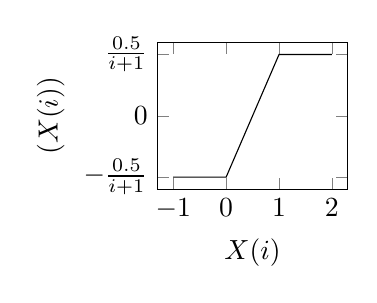
\begin{tikzpicture}[baseline=0.8cm]
        \begin{axis}[width=4cm,xlabel={$X(i)$},xtick={-1,0,1,2},ylabel={$\clipfn(X(i))$},ytick={-0.5,0,0.5},yticklabels={$-\frac{0.5}{i+1}$,$0$,$\frac{0.5}{i+1}$}]
            \addplot[mark=none,samples at={-1,0,1,2}] { min(0.5, x-0.5)-min(0,x) };
        \end{axis}
    \end{tikzpicture}\]

Observe that $\clipfn(C_2(i)-C_1(i)+0.5)$ equals $\frac{0.5}{i+1}$ if $C_1(i)\leq C_2(i)$, and $-\frac{0.5}{i+1}$ otherwise.
This is because the counts $C_1(i),C_2(i)$ must be integers, so if $C_1(i)\leq C_2(i)$, then $C_2(i)-C_1(i)+0.5\geq 0.5$, and the expression will evaluate to $\frac{0.5}{i+1}$. Otherwise, $C_2(i)-C_1(i)+0.5<-0.5$, and the expression will evaluate to $-\frac{0.5}{i+1}$.

It is straightforward, then, to use the construction for $\min$/$\max$ from above to produce a feed-forward layer that computes $\clipfn\left(C_2(i)-C_1(i)\right)$. Essentially, we use $W_1$ to compute the values (using the pre-existing values from the residual stream)

\[\frac{0.5}{i+1}, \frac{C_2(i)-C_1(i)+0.5}{i+1}, -\frac{C_2(i)-C_1(i)+0.5}{i+1}\]

Then we use $W_2$ to compute

\[\frac{0.5}{i+1}+\ReLU\left(\frac{0.5}{i+1}-\frac{C_2(i)-C_1(i)+0.5}{i+1}\right)-\ReLU\left(\frac{0.5}{i+1}-\frac{C_2(i)-C_1(i)-0.5}{i+1}\right)\]
which equals $\clipfn(C_2(i)-C_1(i))$ as desired.

Similarly, it is straightforward to construct a feed-forward layer to compare linear combinations of count terms. That is, for disjoint sets of indices $K_1$ and $K_2$, to compute
\[\clipfn\left(\sum_{k\in K_2} c_{k} \cdot C_k(i) -\sum_{k\in K_1} c_{k} \cdot C_k(i)\right).\]

So we can construct a feed-forward layer $f:\R^d\to\R^d$ that computes in each dimension $i$ the following

\[f\left(\begin{bmatrix}
            v_1        \\
            v_2        \\
            \vdots     \\
            v_{2k_3-1} \\
            v_{2k_3}   \\
            \vdots     \\
            v_{d-1}    \\
            v_{d}      \\
        \end{bmatrix}\right) =\begin{bmatrix}
        \clipfn(v_1)                                                                               \\
        \clipfn(v_2)                                                                               \\
        \vdots                                                                                     \\
        \clipfn\left(\sum_{k\in K_2} c_{k} \cdot C_k(i) -\sum_{k\in K_1} c_{k} \cdot C_k(i)\right) \\
        \clipfn\left(\sum_{k\in K_2} c_{k} \cdot C_k(i) -\sum_{k\in K_1} c_{k} \cdot C_k(i)\right) \\
        \vdots                                                                                     \\
        \clipfn(v_{d-1})                                                                           \\
        \clipfn(v_{d})                                                                             \\
    \end{bmatrix}. \]

This truncates all positive values in the residual stream at this point to be $\frac{0.5}{i+1}$ at position~$i$, and all nonpositive values to be $-\frac{0.5}{i+1}$. As a result, the next application of LayerNorm (with appropriate parameter settings) scales every single value to $\pm 1$. In particular, all previously-computed Boolean values are preserved, and the newly-computed dimensions $2k_3-1,2k$ hold the correct Boolean value based on the desired comparison